%package list
\documentclass{article}
\usepackage[top=3cm, bottom=3cm, outer=3cm, inner=3cm]{geometry}
\usepackage{multicol}
\usepackage{graphicx}
\usepackage{url}
%\usepackage{cite}
\usepackage{hyperref}
\usepackage{array}
%\usepackage{multicol}
\newcolumntype{x}[1]{>{\centering\arraybackslash\hspace{0pt}}p{#1}}
\usepackage{natbib}
\usepackage{pdfpages}
\usepackage{multirow}
\usepackage[normalem]{ulem}
\useunder{\uline}{\ul}{}
\usepackage{svg}
\usepackage{xcolor}
\usepackage{listings}
\lstdefinestyle{ascii-tree}{
    literate={├}{|}1 {─}{--}1 {└}{+}1 
  }
\lstset{basicstyle=\ttfamily,
  showstringspaces=false,
  commentstyle=\color{red},
  keywordstyle=\color{blue}
}
%\usepackage{booktabs}
\usepackage{caption}
\usepackage{subcaption}
\usepackage{float}
\usepackage{array}

\newcolumntype{M}[1]{>{\centering\arraybackslash}m{#1}}
\newcolumntype{N}{@{}m{0pt}@{}}


%%%%%%%%%%%%%%%%%%%%%%%%%%%%%%%%%%%%%%%%%%%%%%%%%%%%%%%%%%%%%%%%%%%%%%%%%%%%
%%%%%%%%%%%%%%%%%%%%%%%%%%%%%%%%%%%%%%%%%%%%%%%%%%%%%%%%%%%%%%%%%%%%%%%%%%%%
\newcommand{\itemGroup}{Grupo B}
\newcommand{\itemCourse}{Programación Web 2}
\newcommand{\itemCourseCode}{1702122}
\newcommand{\itemSemester}{III}
\newcommand{\itemUniversity}{Universidad Nacional de San Agustín de Arequipa}
\newcommand{\itemFaculty}{Facultad de Ingeniería de Producción y Servicios}
\newcommand{\itemDepartment}{Departamento Académico de Ingeniería de Sistemas e Informática}
\newcommand{\itemSchool}{Escuela Profesional de Ingeniería de Sistemas}
\newcommand{\itemAcademic}{2023 - A}
\newcommand{\itemInput}{Del 26 Julio 2023}
\newcommand{\itemOutput}{Al 03 Julio 2023}
\newcommand{\itemPracticeNumber}{08}
\newcommand{\itemTheme}{Django Rest Framework}
%%%%%%%%%%%%%%%%%%%%%%%%%%%%%%%%%%%%%%%%%%%%%%%%%%%%%%%%%%%%%%%%%%%%%%%%%%%%
%%%%%%%%%%%%%%%%%%%%%%%%%%%%%%%%%%%%%%%%%%%%%%%%%%%%%%%%%%%%%%%%%%%%%%%%%%%%

\usepackage[english,spanish]{babel}
\usepackage[utf8]{inputenc}
\AtBeginDocument{\selectlanguage{spanish}}
\renewcommand{\figurename}{Figura}
\renewcommand{\refname}{Referencias}
\renewcommand{\tablename}{Tabla} %esto no funciona cuando se usa babel
\AtBeginDocument{%
	\renewcommand\tablename{Tabla}
}

\usepackage{fancyhdr}
\pagestyle{fancy}
\fancyhf{}
\setlength{\headheight}{30pt}
\renewcommand{\headrulewidth}{1pt}
\renewcommand{\footrulewidth}{1pt}
\fancyhead[L]{\raisebox{-0.2\height}{
\includegraphics[width=3cm]{img/logo_episunsa.png}}}
\fancyhead[C]{\fontsize{7}{7}\selectfont	\itemUniversity \\ \itemFaculty \\ \itemDepartment \\ \itemSchool \\ \textbf{\itemCourse}}
\fancyhead[R]{\raisebox{-0.2\height}{
\includegraphics[width=1.2cm]{img/logo_abet.png}}}
\fancyfoot[L]{\itemTheme}
\fancyfoot[C]{\itemCourse}
\fancyfoot[R]{Página \thepage}

% para el codigo fuente
\usepackage{listings}
\usepackage{color, colortbl}
\definecolor{dkgreen}{rgb}{0,0.6,0}
\definecolor{gray}{rgb}{0.5,0.5,0.5}
\definecolor{mauve}{rgb}{0.58,0,0.82}
\definecolor{codebackground}{rgb}{0.95, 0.95, 0.92}
\definecolor{tablebackground}{rgb}{0.8, 0, 0}

\lstset{frame=tb,
	language=bash,
	aboveskip=3mm,
	belowskip=3mm,
	showstringspaces=false,
	columns=flexible,
	basicstyle={\small\ttfamily},
	numbers=none,
	numberstyle=\tiny\color{gray},
	keywordstyle=\color{blue},
	commentstyle=\color{dkgreen},
	stringstyle=\color{mauve},
	breaklines=true,
	breakatwhitespace=true,
	tabsize=3,
	backgroundcolor= \color{codebackground},
}

\begin{document}
	
	\vspace*{10px}
	
	\begin{center}	
		\fontsize{17}{17} \textbf{ Informe de Laboratorio \itemPracticeNumber}
	\end{center}
	\centerline{\textbf{\Large Tema: \itemTheme}}
	%\vspace*{0.5cm}	

	\begin{flushright}
		\begin{tabular}{|M{2.5cm}|N|}
			\hline 
			\rowcolor{tablebackground}
			\color{white} \textbf{Nota}  \\
			\hline 
			     \\[30pt]
			\hline 			
		\end{tabular}
	\end{flushright}	

	\begin{table}[H]
		\begin{tabular}{|x{4.7cm}|x{4.8cm}|x{4.8cm}|}
			\hline 
			\rowcolor{tablebackground}
			\color{white} \textbf{\itemGroup} & \color{white}\textbf{Escuela}  & \color{white}\textbf{Asignatura}   \\
			\hline 
			{\begin{itemize}
				\item Ccahuana Larota, Joshep Antony \item Christian Zapana Romero, Pedro Luis \item Mejia Ramos, Piero Douglas
			\end{itemize}} & 
			{\begin{center}\itemSchool \end{center}} & 
			{\begin{center}\itemCourse \par Semestre: \itemSemester \par Código: \itemCourseCode \end{center}}     \\
			\hline 			
		\end{tabular}
	\end{table}		
	
	\begin{table}[H]
		\begin{tabular}{|x{4.7cm}|x{4.8cm}|x{4.8cm}|}
			\hline 
			\rowcolor{tablebackground}
			\color{white}\textbf{Laboratorio} & \color{white}\textbf{Tema}  & \color{white}\textbf{Duración}   \\
			\hline 
			\itemPracticeNumber & \itemTheme & 04 horas   \\
			\hline 
		\end{tabular}
	\end{table}
	
	\begin{table}[H]
		\begin{tabular}{|x{4.7cm}|x{4.8cm}|x{4.8cm}|}
			\hline 
			\rowcolor{tablebackground}
			\color{white}\textbf{Semestre académico} & \color{white}\textbf{Fecha de inicio}  & \color{white}\textbf{Fecha de entrega}   \\
			\hline 
			\itemAcademic & \itemInput &  \itemOutput  \\
			\hline 
		\end{tabular}
	\end{table}
	
	\section{Competencias del curso}
	
	\begin{itemize}
		\item General: C.c. Diseña responsablemente aplicaciones web, sus componentes o procesos para satisfacer necesidades dentro de restricciones realistas: económicas, medioambientales, sociales, políticas, éticas, de salud, de seguridad, manufacturación y sostenibilidad.
		\item Específica: C.m. Construye responsablemente soluciones con tecnología web siguiendo un proceso adecuado llevando a cabo las pruebas ajustada a los recursos disponibles del cliente.
		\item C.p. Aplica de forma flexible técnicas, métodos, principios, normas, estándares y herramientas del desarrollo web necesarias para la construcción de aplicaciones web e implementación de estos sistemas en una organización.
	\end{itemize}
	
	\section{Resultado del estudiante}
	
	\begin{itemize}
		\item RE. 2 La capacidad de aplicar diseño de ingeniería para producir soluciones a problemas y diseñar sistemas, componentes o procesos para satisfacer necesidades específicas dentro de consideraciones realistas en los aspectos de salud pública, seguridad y bienestar; factores globales, culturales, sociales, económicos y ambientales.
		\item RE. 8 La capacidad de crear, seleccionar y utilizar técnicas, habilidades, recursos y herramientas modernas de ingeniería y tecnologías de la información, incluyendo la predicción y el modelado, con una comprensión de las limitaciones.
		
	\end{itemize}
	
	\section{Equipos, materiales y temas}
	
	\begin{itemize}
		\item Sistema Operativo (GNU/Linux de preferencia).
		\item GNU Vim.
		\item Python 3.
		\item Git.
		\item Cuenta en GitHub con el correo institucional.
		\item Entorno virtual.
		\item Django 4.
		\item Django REST framework.
	\end{itemize}
	
	\section{Marco teórico}
	
	\subsection{Django Rest Framerowk:}
	
	\begin{itemize}
		\item Django REST framework es un conjunto de herramientas potente y flexible para crear API web.
		\item Algunas razones por las que podrías querer usar el marco REST:
		
		\begin{itemize}
			\item La API navegable por la Web es una gran ganancia de usabilidad para sus desarrolladores.
			\item Políticas de autenticación que incluyen paquetes para OAuth1 y OAuth2.
			\item Serialización que admite fuentes de datos ORM y no ORM.
			\item Personalizable hasta el final: solo use las vistas regulares basadas en funciones si no necesita las funciones más potentes.
			\item Amplia documentación y gran apoyo de la comunidad.
			\item Utilizado y confiado por empresas reconocidas internacionalmente, como Mozilla, Red Hat, Heroku y Eventbrite.
		\end{itemize}
		
	\end{itemize}
	
	\section{Tarea}
	
	\begin{itemize}
		\item Elabore un servicio web que tenga un CRUD con el uso de este framework.
		
		\begin{itemize}
			\item \textbf{Create} - \textit{POST}
			\item \textbf{Read} - \textit{GET}
			\item \textbf{Update} - \textit{PUT}
			\item \textbf{Delete} - \textit{DELETE}
		\end{itemize}
		
		\item Centrarse en el Core business de su aplicación web. Lo más importante y necesario debe estar disponible a través de un servicio web. A continuación, se presentan algunos ejemplos de servicios web:
		
		\begin{itemize}
			\item \url{https://reqbin.com/}
			\item \url{https://www.googleapis.com/youtube/v3/playlistItems}
		\end{itemize}
		
		\item Muestre la funcionalidad consumiéndola desde el cliente REST de su preferencia. El método \textit{GET} puede ser directamente consumido por un navegador web. Por ejemplo, en esta API se puede obtener la temperatura de Arequipa en un rango de fechas (la versión gratuita tiene un retraso de 7 días, por tanto, solo mostrará la temperatura en Arequipa desde el 01 de Julio hasta el 03 de Julio): 
		
		\item \url{https://archive-api.open-meteo.com/v1/archive?latitude=-16.39889&longitude=-71.535&start_date=2023-07-01&end_date=2023-07-10&hourly=temperature_2m&daily=temperature_2m_max,temperature_2m_min&timezone=America%2FNew_York}
		
	\end{itemize}

	\section{Desarrollo}
	
	\subsection{Proyecto}
	
	Para está sección se presenta las configuraciones en los módulos settings.py y urls.py de la carpeta "library" dek proyecto "library":
	
	\subsubsection{settings.py}
	
	Se agrega la aplicación reservation, books, y el rest\_framework.
	
	\lstinputlisting[language=Python, caption={settings.py},numbers=left,]{src/settings1.py}
	
	Ademas de la modificación al directorio de busqueda para los templates:

	
	\lstinputlisting[language=Python, caption={settings.py},numbers=left,]{src/settings2.py}

	\subsubsection{urls.py}
	
	En está sección se ve la implementación de la url api
	
	\lstinputlisting[language=Python, caption={urls.py},numbers=left,]{src/urls.py}
	
	
	\subsection{Aplicación reservation}
	
	En está sección se mostrara la configuración y la funcionalidad de cada módulo usado en la palicación.
	
	\subsubsection{admin.py}
	
	El código en el archivo admin.py de la aplicación "reservation" registra los modelos "Libro" y "User" para que puedan ser administrados desde la interfaz de administración de Django. La función 
	admin.site.register(Modelo) se utiliza para registrar un modelo en la interfaz de administración.
	
	Una vez que los modelos están registrados, podrán ser gestionados (crear, leer, actualizar y eliminar objetos) desde la interfaz de administración en el navegador, siempre y cuando se tenga acceso como usuario con privilegios de administrador o superusuario. Recuerda que antes de desplegar la aplicación en producción, es esencial implementar la autenticación y autorización adecuadas para proteger el acceso a la interfaz de administración y los datos de la base de datos.
	
	\lstinputlisting[language=Python, caption={admin.py},numbers=left,]{src/admin.py}
	
	
	
	\subsubsection{models.py}
	
	
	\begin{enumerate}
		\item Libro
		
		\begin{itemize}
			\item Tiene cuatro campos: "nombre", "author", "codigo", y "img" (imagen).
			\item Los campos "nombre" y "author" son cadenas de caracteres con una longitud máxima de 50 caracteres.
			\item  El campo "codigo" es un entero que almacena un número.
			\item El campo "img" es una imagen que se almacena en el directorio "pics" dentro del sistema de archivos.
			\item También tiene un campo adicional "desc" (descripción), que es un campo de texto que puede almacenar una descripción del libro.
			\item El método \_\_str\_\_() se ha definido para que al imprimir un objeto "Libro", se muestre su nombre.
		\end{itemize}
		
		\item User
		\begin{itemize}
			\item Tiene cuatro campos: "nombre", "email", "deuda", y "libroPrest".
			\item Los campos "nombre" y "email" son cadenas de caracteres con una longitud máxima de 50 caracteres.
			\item  El campo "deuda" es un booleano que indica si el usuario tiene una deuda o no, con un valor predeterminado de "False".
			\item El campo "libroPrest" es una clave externa (ForeignKey) que establece una relación entre el modelo "User" y el modelo "Libro". Indica que un usuario puede tener varios préstamos de libros, y se define con el argumento "on\_delete=models.CASCADE", lo que significa que si se elimina un libro relacionado, también se eliminarán los préstamos asociados a ese libro.
			\item El método \_\_str\_\_() se ha definido para que al imprimir un objeto "User", se muestre su nombre.
		\end{itemize}
	\end{enumerate}
	
	\lstinputlisting[language=Python, caption={models.py},numbers=left,]{src/models.py}
	
	En resumen, estos modelos definen la estructura de datos para los libros y los usuarios en la aplicación, y permiten almacenar y gestionar información relacionada con los libros disponibles y los préstamos realizados por los usuarios.
	
	
	\subsubsection{serialiers.py}
	
	El código proporciona dos clases llamadas LibroSerializer y UserSerializer, que son utilizadas para convertir los objetos de los modelos Libro y User en formatos que se pueden enviar a través de la web o almacenar en una base de datos.\\
	
	En términos sencillos, estas clases son "traductores" que toman los datos de los objetos de los modelos Libro y User y los convierten en una estructura que puede ser fácilmente entendida y procesada por aplicaciones que utilicen el framework Django REST.\\
	
	Para ser más precisos:
	
	\begin{itemize}
		\item LibroSerializer se encarga de tomar un objeto de la clase Libro y convertirlo en un formato de datos que incluye los campos url, nombre, author, codigo, img y desc.
		\item  UserSerializer toma un objeto de la clase User y lo convierte en un formato que contiene los campos url, nombre, email, deuda y libroPrest.
	\end{itemize}
	
	Estas clases son parte del módulo rest\_framework de Django y son esenciales cuando se trabaja con API RESTful, ya que permiten serializar y deserializar datos entre las representaciones internas de los objetos y los formatos que se envían a través de la web, como JSON o XML. De esta manera, se facilita la comunicación entre el servidor y el cliente al procesar datos en diferentes formatos.\\
	
	\lstinputlisting[language=Python, caption={serializers.py},numbers=left,]{src/serializers.py}
	
	\subsubsection{urls.py}
	
	El código configura las URL para un servicio web utilizando Django REST Framework. Se importan las funciones y clases necesarias desde los módulos de Django, como \texttt{path} para definir rutas URL y \texttt{include} para incluir otras rutas URL desde otras aplicaciones. Se crea una instancia de \texttt{DefaultRouter} llamada \texttt{router}, que preconfigura las rutas comunes para un conjunto de vistas, facilitando la generación de URL para operaciones CRUD. Se registran las vistas \texttt{LibroViewSet} y \texttt{UserViewSet} con sus respectivas rutas en el \texttt{router}. La variable \texttt{urlpatterns} contiene las rutas URL que se utilizarán para acceder a las vistas de la API, incluyendo las rutas proporcionadas por el \texttt{router}.\\
	
	En resumen, el código establece las rutas de acceso a diferentes vistas de la API mediante el uso de \texttt{DefaultRouter} de Django REST Framework.
	
	\lstinputlisting[language=Python, caption={urls.py},numbers=left,]{src/urls.py}
	
	
	
	\subsubsection{views.py}
	
	El código proporciona vistas (\textit{views}) para un servicio web utilizando Django REST Framework. Se importan funciones y clases necesarias, incluyendo \texttt{render}, modelos \texttt{Libro} y \texttt{User}, y clases \texttt{viewsets} y \texttt{permissions} de Django REST Framework, junto con los serializadores\\ \texttt{LibroSerializer} y \texttt{UserSerializer}.\\
	
	Se definen dos clases de vistas: \texttt{LibroViewSet} y \texttt{UserViewSet}, que heredan de\\ \texttt{viewsets.ModelViewSet}. Estas clases representan vistas basadas en modelos que brindan funcionalidades CRUD para los modelos \texttt{Libro} y \texttt{User}.\\
	
	Dentro de cada clase de vista, se definen tres atributos:
	\begin{itemize}
		\item \texttt{queryset}: Especifica el conjunto de objetos que se utilizarán en la vista. Para la vista\\ \texttt{LibroViewSet}, se trabaja con todos los objetos de la clase \texttt{Libro}.
		\item \texttt{serializer\_class}: Indica el serializador que se utilizará para convertir los objetos del modelo en representaciones JSON y viceversa. Para la vista \texttt{LibroViewSet}, se utiliza \texttt{LibroSerializer}, y para la vista \texttt{UserViewSet}, se utiliza \texttt{UserSerializer}.
		\item \texttt{permission\_classes}: Define las clases de permisos requeridas para acceder a la vista. Se requiere que el usuario esté autenticado para acceder a ambas vistas, por lo que se utiliza\\ \texttt{permissions.IsAuthenticated}.
	\end{itemize}
	
	\lstinputlisting[language=Python, caption={views.py},numbers=left,]{src/views.py}
	
	
	\subsection{Base HTML}
	
	\lstinputlisting[language=HTML, caption={index.html},numbers=left,]{src/index.html}
	
	
	\section{Ejecución}
	
	\begin{figure}[h]
		\centering
		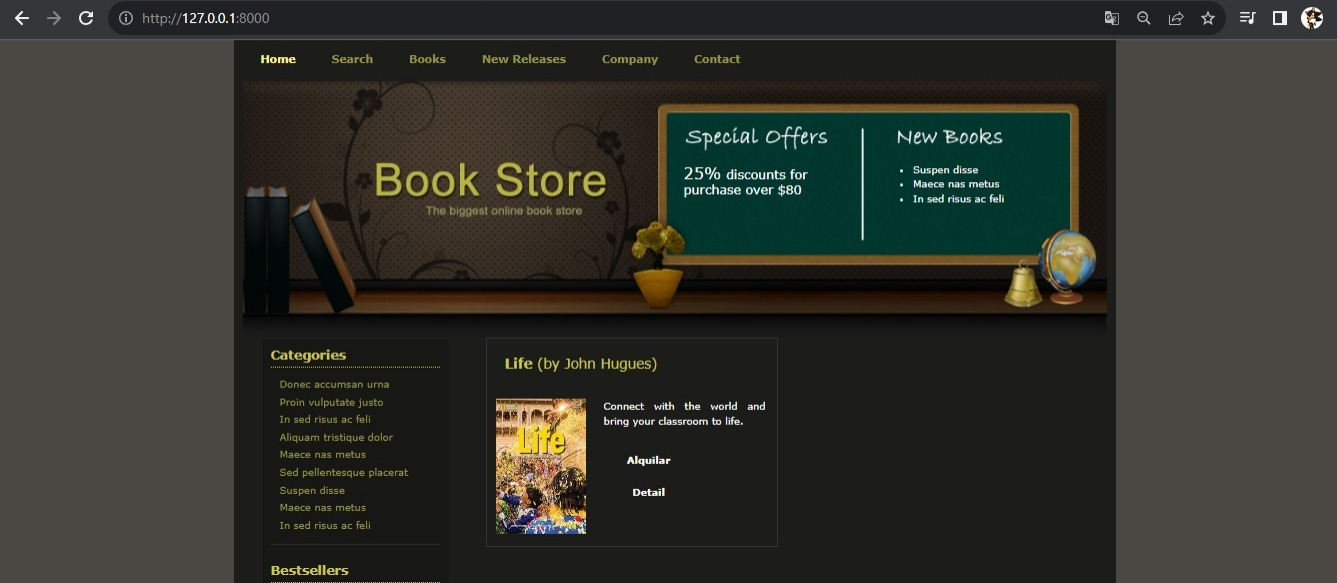
\includegraphics[width=\textwidth]{img/htmlbase.jpeg}
		\caption{Html basico}
	\end{figure}
	
	\begin{figure}[h]
		\centering
		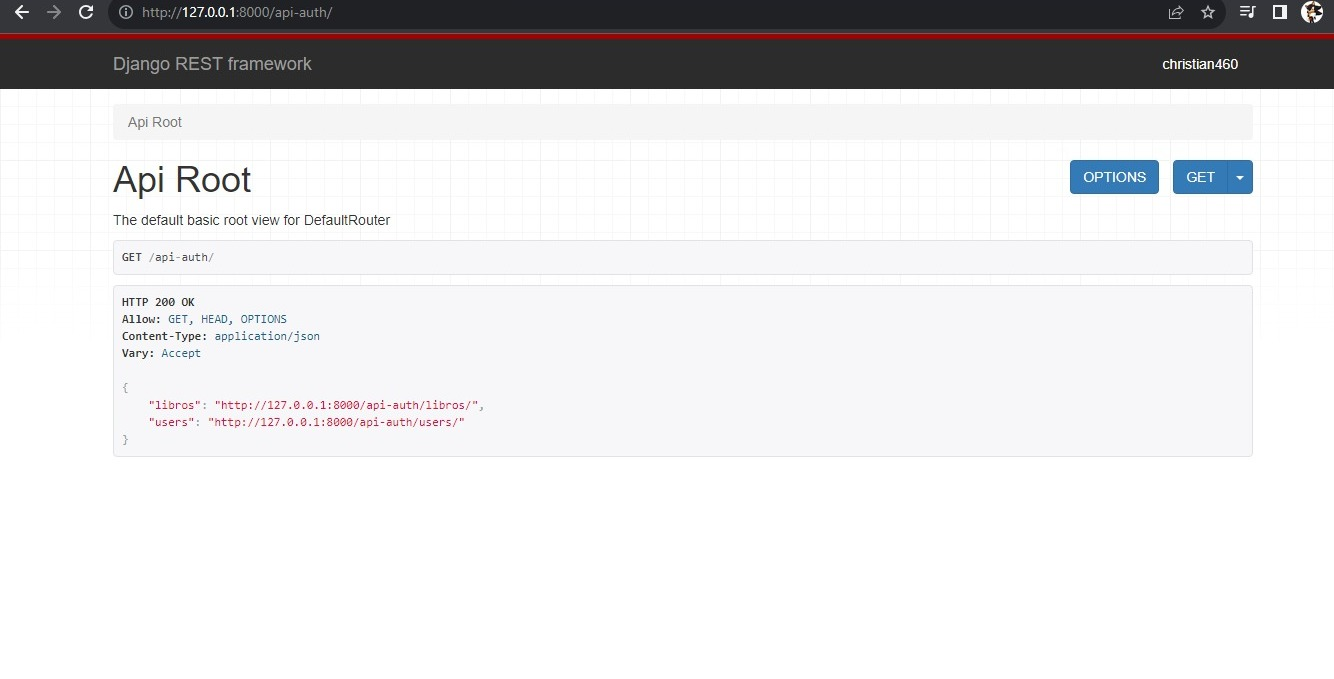
\includegraphics[width=\textwidth]{img/api-auth.jpeg}
		\caption{api-auth}
	\end{figure}
	
	\begin{figure}[h]
		\centering
		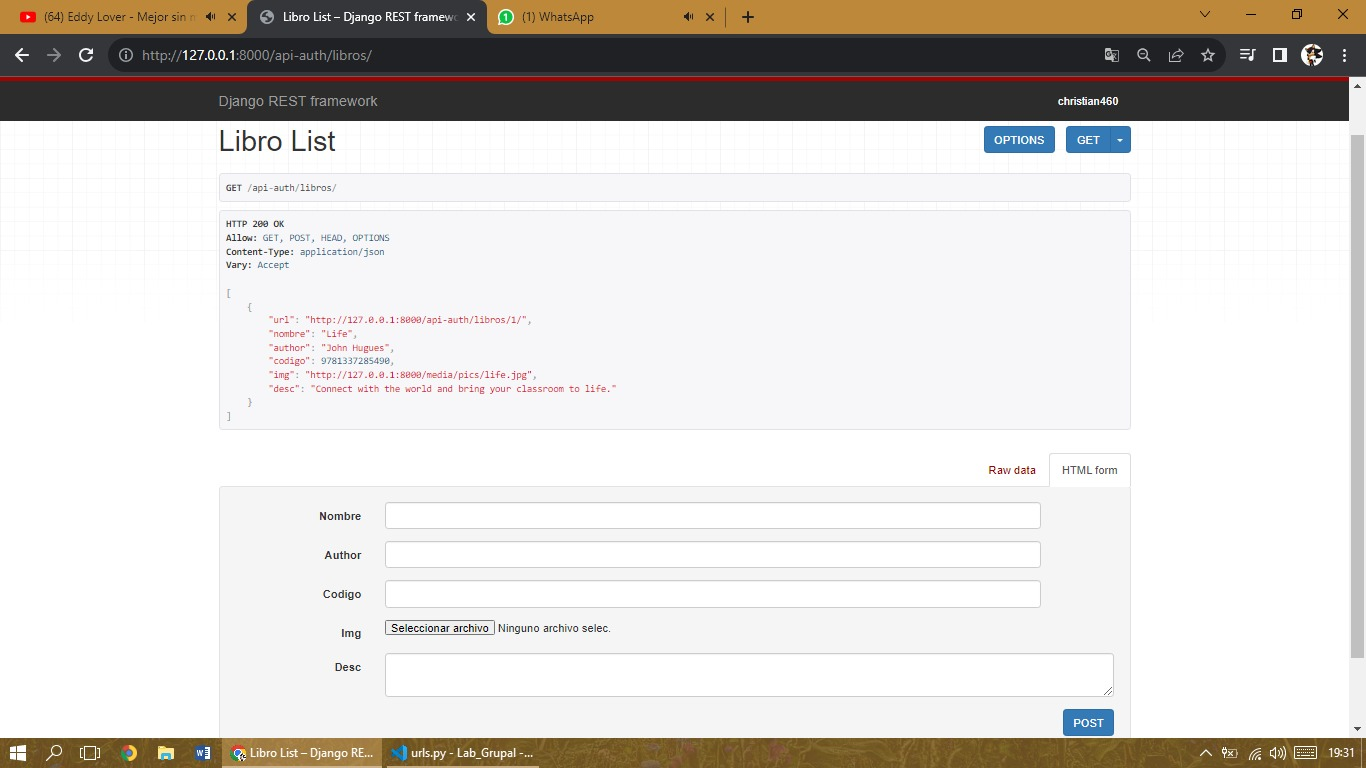
\includegraphics[width=\textwidth]{img/api-auth-libros.jpeg}
		\caption{Lista de libros}
	\end{figure}
	
	
	\section{Pregunta}
	
	\begin{itemize}
		\item ¿Cuál fué la mayor dificultad del uso de este framework?\\
		La mayor dificultad sería útil izar el renderizador para poder utilizar los modelos.
	\end{itemize}
	
	\section{URL de Repositorio Github}
	
	\url{https://github.com/christian460/Lab_Grupal.git}
	
	\section{URL de Referencias}
	
	\begin{itemize}
		\item \url{https://www.django-rest-framework.org/}
		\item \url{https://www.django-rest-framework.org/tutorial/quickstart/}
		\item \url{https://www.django-rest-framework.org/tutorial/1-serialization/}
		\item \url{https://www.django-rest-framework.org/tutorial/3-class-based-views/}
		\item \url{https://www.django-rest-framework.org/api-guide/authentication/}
		\item \url{https://www.bezkoder.com/django-rest-api/}
	\end{itemize}
	
\end{document}
